% !TEX root = ../main.tex
\section{Introductory Remarks}

The blockchain data structure and consensus mechanism has received significant interest since being introduced as the underlying technology of the cryptocurrency Bitcoin in Satoshi Nakamoto's (pseudonymous) 2008 whitepaper~\cite{nakamoto2008bitcoin}. In 2014, Buterin presented a new blockchain based application known as Ethereum~\cite{buterin2014next}. As a blockchain-based distributed public network, Ethereum implements a decentralized virtual machine, known as the Ethereum Virtual Machine (EVM), which allows network nodes to execute deployed programmable smart contracts on the Ethereum blockchain~\cite{wood2014ethereum}.This platform enables developers to create and execute blockchain applications called \textit{decentralized applications (dapps)} that are executed correctly according to the consensus of the network. A Dapp's code and data is stored in a decentralized manner on the blockchain. Dapps or smart contracts are now often written in a high level programming language such as \textit{Solidity} which is syntactically similar to Java~\cite{Ethereum41:online}. Digital smart contracts were first described Nick Szabo in 1993~\cite{szabo1997formalizing}, however they reached a high level of adoption through blockchain technology.

One application of blockchain technology that has received some research and commercial interest is the idea of replacing (or augmenting) the web certificate model used by clients (OS and browsers) to form secure communication channels with web-servers (described in more detail below). This model has been plagued with issues from fraudulent certificates used to impersonate servers to ineffective revocation mechanisms; see Clark and van Oorschot for a survey~\cite{CO13}. We argue that the application of blockchains to this model is more than an interesting experiment; it is actually a new \UA paradigm that resolves some of the fundamental issues with the current model --- authority and indirection. We also argue that adding programmability to a dapp-based PKI provides benefits beyond using the blockchain as an append-only broadcast channel. Finally, we instantiate our ideas in a novel system called \Ghazal implemented in Solidity and deployed on Ethereum. At the time of writing, the overall system costs under \$100 to deploy. Basic actions like domain registration costs under \$5. 

% = = = = = = = = = = = = = = = = = = = = = = = = = = = = = = = = = = = = = = = = = =

\section{Related Work}

The HTTPS (HTTP over SSL/TLS) protocol enables secure connections to websites with confidentiality, message integrity, and server authentication. Server authentication relies on a client being able to determine the correct public key for a server. The current web certificate model uses a system of certificate authorities (CAs); businesses that provide this binding in the form of a certificate. Client devices, through the browser and/or the operating system, are pre-installed with a set of known CAs who can delegate authority to intermediary CAs through a protocol involving certificates. When a CA issues a certificate to a web-server, there are generally three types: domain validated (DV) certificates bind a public key only to a domain (\eg \texttt{example.com}), while organization validated (OV) and extended validated (EV) certificates validate additional information about the organization that operates the server (Example, Inc.).

Namecoin is an altcoin (software based on Bitcoin with a distinct blockchain) that implements a decentralized namespace for domain names~\cite{Kalodner2015}. The main feature of Namecoin is that for a fee, users can register a \texttt{.bit} address and map it to an IP address of their choice.  CertCoin~\cite{fromknecht2014certcoin}, and PB-PKI~\cite{axon2016pb} are extensions to Namecoin that add the ability to specify an HTTPS public key certificate for the domain (as well as other PKI operations like expiration and revocation, which we discuss in Section~\ref{sec:revocation}). Blockstack~\cite{ali2016blockstack} achieves the same goal by embedding data into a root blockchain, a process called virtualchains that could be instantiated with \texttt{OP\_RETURN} on Bitcoin's blockchain. These approaches are closest to our own system \Ghazal. These systems disintermediate CAs from the web certificate model. The main difference is that we use Ethereum to provide full programmability (motivated below in Section~\ref{sec:program}). In addition, we provide some minor improvements such as allowing multiple keys to be bound to the same domain, as is common for load balancing and CDNs.

Some research has looked at adding transparency, effectively through an efficient log of CA-issued certificates, to augment the current web certificate model. This is a very active area of research that includes certificate transparency (CT)~\cite{laurie2014certificate}, sovereign keys (SKs)~\cite{giteffor4:online}, and ARPKI~\cite{basin2014arpki}. IKP~\cite{matsumoto2016ikp} provides an Ethereum-based system for servers to advertise policies about their certificates (akin to a more verbose CAA on a blockchain instead via DNS). Research a bit further removed from web certificates concerns decentralized PKIs and broader identities. While not decentralized, CONIKS provides a distributed transparency log similar to CT but for public keys (while they could be for anything, email and IM are the primary motivations)~\cite{melara2015coniks}. Bonneau provides an Ethereum smart contract for monitoring CONIKS~\cite{bonneau2016ethiks}. ClaimChain is similar to CONIKS but finds a middle-ground between a small set of distributed servers (CONIKS) and a fully decentralized but global state (blockchain) by having fully decentralized, local states that can be cross-validated. CONIKS and ClaimChain do not use CAs but rather rely on users validating the logs, which are carefully designed to be non-equivocating. ChainAnchor provides identity and access management for private blockchains~\cite{hardjonoverifiable}, while CoSi is a distributed signing authority generic logging~\cite{syta2016keeping}. Each of these systems is concerned with logging data (a generic umbrella that encapsulates many of these is Transparency Overlays~\cite{chase2016transparency}). As logging systems, they do not provide programmability which is the primary motivation for our system. 

Finally, some research has explored having public validated by external parties but replacing the role of CAs with a PGP-style web of trust. SCPKI is an implementation of this idea on Ethereum~\cite{al2017scpki}. Our observation is that for domain validation, a blockchain with a built-in naming system is already authoritative over the namespace and does not require additional validation. 

% = = = = = = = = = = = = = = = = = = = = = = = = = = = = = = = = = = = = = = = = = =

\section{Motivation}

\subsection{Are Blockchains a new paradigm for PKI?}

In the related work, most blockchain-approaches to identity (or specifically PKI) motivate their approach with Zooko's triangle; an articulation of three natural properties one might want from an identity system: memorable names, secure (as in hard to impersonate), and a distributed authority for issuing names. His assertion is that two of the three properties can be achieved effortlessly but adding the third is difficult or impossible. Blockchains, starting with Namecoin for domain names and extensions to PKI, are often claimed to resolve this trilemma enabling all three properties in one system. A blockchain is  distributed, short human-friendly names can be claimed by anyone, and ownership over a name is secured with a strong cryptographic key. 

We approach thinking about this issue a little differently. In the current web certificate model, certificate authorities are meant to be $authorities$: that is, they are authoritative over the namespace they bind keys to. The reality is that the web still runs largely on domain validated certificates~\cite{DKBH13,HBKC11} and for domain validation, certificate authorities are not any more or less authoritative over who owns what domain than you or I. Certificate authorities instead rely on indirection. For example, a certificate authority might validate a request by Alice for a certificate for \texttt{alice.com} by sending an email to \texttt{admin@alice.com} with a secret nonce that Alice must type into a webform. This involves 2 levels of indirection: (1) CAs appeal to DNS to establish the MX record of the domain (\ie the subscriber's mail server's IP address); (2) CAs appeal to SMTP to establish a communication channel to the subscriber. For each level of indirection, there are a set of vulnerabilities which might allow a malicious party to break the verification process and obtain a fraudulent certificate for a domain they do not own. For example, consider the attack surface of email-based validation:

\begin{enumerate}

\item \textbf{Reserved Emails:} A CA specifies a list of email addresses to receive the challenge. The underlying assumption is that only the domain owner controls this address. However the domain owner might not reserve that email address or even be aware that a certain email address is being used by one of the CAs for this purpose. And recall that just a single CA needs to use a single non-standard email address (\eg a translation of administrator into their local language) to open up this vulnerability. For example, Microsoft's public webmail service \texttt{login.live.com} saw an attacker successfully validate his ownership of the domain using an email address \texttt{sslcertificates@live.com} which was open to public registration~\cite{zusman2009criminal}.

\item \textbf{Whois Emails:} A CA also optionally draws the email address from the Whois record for the domain. A domain's whois record is generally protected by the username/password set by the domain owner with their registrar. Any attack on this password (\eg guessing or resetting) or directly on the account (\eg social engineering~\cite{GoDaddyo45:online}) would allow the adversary to specify an email address that they control. 

\item \textbf{MX Record:} A CA establishes the IP address of the mailserver from the MX record for the domain. As above, all domain records including the MX record is managed through the owner's account with her domain registrar. Any method for obtaining unauthorized access to this account would enable an adversary to list their own server in the MX record and receive the email from the CA.

\item \textbf{DNS Records:} If an adversary cannot directly change a DNS record, they might conduct other attacks on the CA's view of DNS. For example, they might employ DNS cache poisoning which can result in invalid DNS resolution~\cite{son2010hitchhiker}. They might also exploit an available dangling DNS record (Dare)~\cite{liu2016all}. Dares occur when data in a DNS record (such as CNAME, A, or MX) becomes invalid but is not removed by the domain owner. For example, if the domain owner forgets to remove the MX record (the IP address of the server) from DNS, the associated DNS MX record is said to be dangling. If an adversary can acquire this IP address at some future point, he is able to redirect all traffic intended for the original domain to his server, including information sufficient for a CA's domain validation process. Thus a malicious party can use a Dare to obtain a fraudulent certificate. In a \UA system, Dares are still possible (old data that hasn not been purged from the system) but the public keys dangle with the IP address, which resolves the security issue for mis-issued certificates

\item \textbf{SMTP:} Once the CA establishes the mailserver's record, it will send the email to the mailserver with SMTP (the standard protocol for transfer of email). Since the email contains a secret nonce, confidentiality of this email is crucial. SMTP uses opportunistic encryption that is not secure against an active adversary. Thus a man-in-the-middle between the CA's mailserver and the ultimate destination (including an forwarding mailservers) could request a fraudulent certificate, intercept the ensuing email, reply with the correct nonce, and be issued the fraud\-ulent certificate.

\item \textbf{Email Accounts:} Email accounts are generally protected with a username and password (over IMAP or POP3) to prevent unauthorized access. In some cases, they might be protected with a client certificate. An adversary who can gain access to any one of the accounts that should be reserved by the domain owner (\eg texttt{admin}, \texttt{hostmaster}, \texttt{webmaster}, \etc) could obtain a fraudulent certificate for that site. This could include guessing or resetting the password, using social engineering, or obtaining access to the server hosting the email for the account. 

\end{enumerate}


Blockchains are actually a new paradigm; they collapse the indirection for domain validation. If a PKI were added to a blockchain, who would be authoritative over the namespace of domain names? When domain names themselves are issued through the blockchain (\eg Namecoin), then the blockchain is actually the authoritative entity. Arguably, this indirection can be collapsed in the traditional web certificate model as well. There DNS (in conjunction with ICANN) is authoritative over the namespace and if ICANN/DNS held key bindings, there would be no indirection or CAs needed --- indeed, this is exactly the proposal of DANE. Thus blockchains and DANE are both examples of what we might call a \UA paradigm. A deployment issue with DANE is that DNS records do not generally have message integrity (except via the under-deployed DNSSEC) whereas blockchain transactions do. 

%To illustrate the benefits of UA, consider a recent example from the literature~\cite{liu2016all}. Dangling DNS records (Dares) occur when the data in a DNS record (such as CNAME, A, or MX) becomes invalid but is not removed by the domain owner. For example, if the domain owner forgets to remove the A record (the IP address of the server) from DNS, the associated DNS A record is said to be dangling. If an adversary can acquire this IP address at some future point, he is able to redirect all traffic intended for the original domain to his server, including information sufficient for a CA's domain validation process. Thus a malicious party can use a Dare to obtain a fraudulent certificate. In a \UA system, Dares are still possible (old data that hasn't been purged from the system) but the public keys dangle with the IP address, which resolves the security issue for mis-issued certificates.

%
%To illustrate this in more detail, we will consider email-based domain ownership validation. We note that email validation works in conjunction with DNS, so the vulnerabilities on this process subsume the set of vulnerabilities of DNS-based validation. We leave aside HTTP-based validation as it is largely similar; but we note one interesting issue: the CA must fetch the posted hash of the certificate request from the website and since the website is trying to obtain a certificate, it follows that they likely do not have an existing certificate and therefore are not providing this file over HTTPS. Any man-in-the-middle between the webserver and the CA could respond to the CA's request with a fraudulent CSR (even if it doesn't actually exist on the webserver) and obtain a fraudulent certificate. 





\subsection{Does programmability add anything?}
\label{sec:program}

In the related work, some systems take a \UA approach while others rely on third party authorities (generally, CAs or web of trust). Most systems that use a blockchain (or similar trasnparency log) do it in a passive way---as an append-only broadcast channel; a few systems actually use smart contracts or the programmability that a blockchain provides. Of all these systems, to the best of our knowledge, none are both \UA and use programmability. We have argued the merits of uni-authoriatiative above, what about programmability? What does it provide?

Programmability, or PKI bindings within a smart contract, can enable features that seem desirable. A few examples include: external contracts that can easily obtain information about a domain in making decisions; atomonicity within domain name transfers where payments and transfers are inputs to the same transaction (\eg even Namecoin relies on a third party tool called ANTPY to perform atomic name ownership transfer transactions); and fancier options for transfering domain names: we implement an auction where any domain owner can auction off their domain within the smart contract itself. The reader might think of other features that programmability could add.

In defence of non-programmable blockchain-based PKIs, such as Blockstack, it is not clear how well a system like ours scales and what demands it puts on user clients to quickly fetch information on domains. We return to this in the next section, however we note here that we are not claiming programmability necessarily wins out in the end, only that it is worth exploring from a research perspective to better understand the trade-offs. 

% = = = = = = = = = = = = = = = = = = = = = = = = = = = = = = = = = = = = = = = = = =

\section{The \Ghazal System}

Our proposed scheme is entitled \Ghazal, a smart contract-based naming and PKI \UA system. \footnote{\GhazalCode} It enables entities, whether they are people or organizations, to fully manage and maintain control of their domain name without relying on trusted third parties. In \Ghazal, a user can register an unclaimed domain name as a globally readable identifier on the Ethereum blockchain. Subsequently, she is able to assign arbitrary data, such as TLS certificates to her domain. These values are globally readable, non-equivocating, and not vulnerable to the indirection attacks outlined above. The penalty paid for a \UA approach is that \Ghazal has to carve out its own namespace that is not already in use (\eg names ending in \texttt{.ghazal} like Namecoin's \texttt{.bit} or Blockstack's \texttt{.id}). OS and browsers would have to be modified before any system like this can be used. Anyone can claim a domain on a first-come, first-serve basis. Because it is decentralized, names cannot be re-assigned without the cooperation of the owner (whereas an ICANN address like \texttt{davidduchovny.com} can be re-assigned through adminstrative mediation).

The design of \Ghazal consists of two essential elements. First, the smart contract that resides on the Ethereum blockchain and  serves as an  interface between entities and the underlying blockchain. The second primary component of the system are the clients, including people or organizations that interact with \Ghazal smart contract in order to manage their domain names. Figure 1 represents the primary states a domain name can be in and how state transitions work. These states are enforced within the code itself to help mitigate software security issues related to unintended execution paths. 

% ==============State Diagram Figure====================== %
%\begin{figure}[htb!p]
%\centering
%<<<<<<< HEAD
%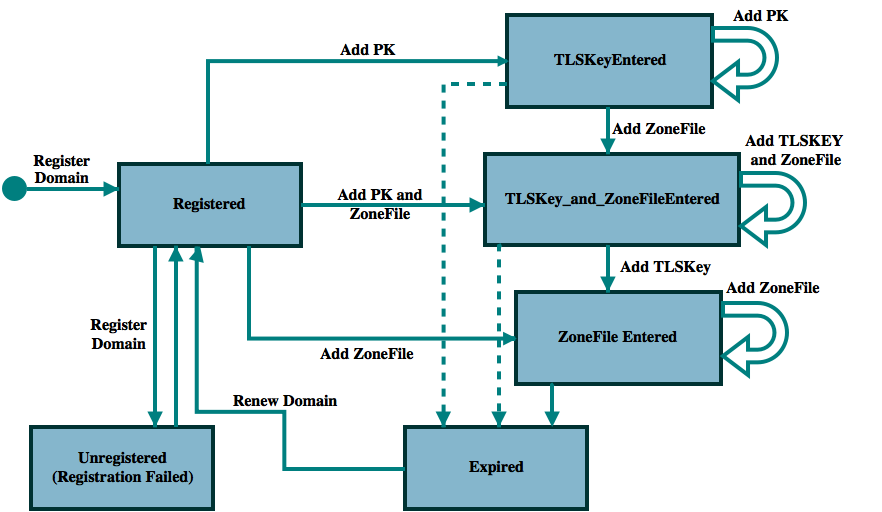
\includegraphics[scale=0.7]{Fig/StateDiagram-2.png}
%=======
%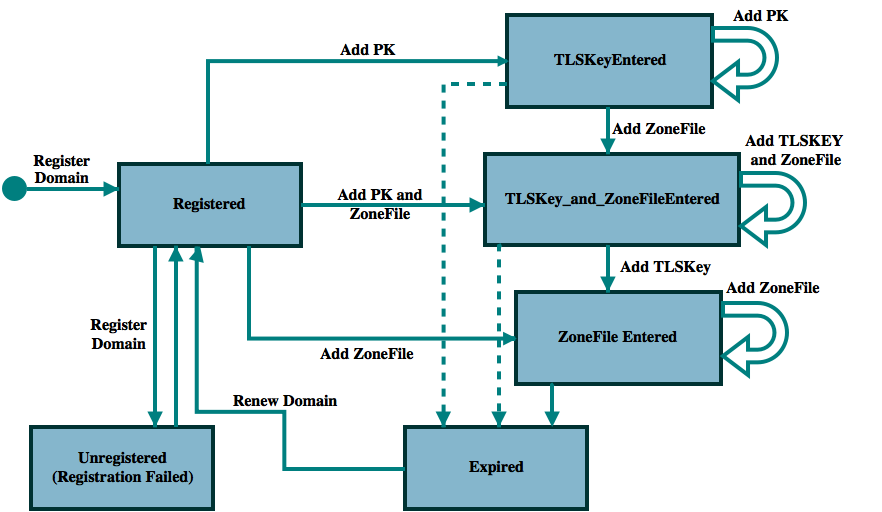
\includegraphics[width=0.9\textwidth]{fig/StateDiagram-2.png}
%>>>>>>> 9b9de7f0a0c50129aee0826714b02e096ce50837
%\caption{\footnotesize{Primary states and transitions for a domain name in \Ghazal.}}
%\end{figure}

\begin{figure}[htb!p]
\centering
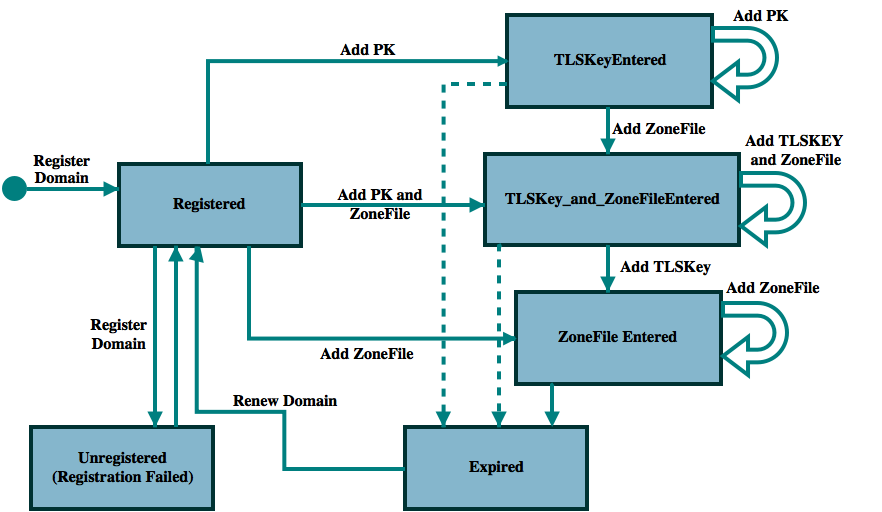
\includegraphics[width=0.9\textwidth]{fig/StateDiagram-2.png}
\caption{\footnotesize{Primary states and transitions for a domain name in \Ghazal.}}
\end{figure}
%===================================================%

\subsection{Exploring \Ghazal design choices}

Beyond simply presenting our design, we think it is useful to explore the landscape of possible designs. To this end, we discuss some deployment issues that we faced where there was no obvious ``one right answer.'' These are likely to be faced by others working in this space (whether working narrowly on PKI or broad identity on blockchain solutions). 

% ==============Design Decision \#1: Domain Name Expiration================= %

\subsubsection{Design Decision \#1: Domain Name Expiration\newline} 

Typically domain name ownership eventually \textit{expires}. Once a domain expires, it is returned to the primary market, except if the users renews it. However, expiration does not necessarily have to mean a disclaimer of ownership; there are other options. 

\begin{enumerate}

\item \textbf{Domain names never expire and last forever.} Designing a system with no domain name expiration would be highly vulnerable to domain squatting. Domain squatting is registering domain names in speculation that the will increase in value. These domain names generally do not point to any relevant IP address (except to earn revenue on accidental visits). If domain names never expire, squatting may be significantly problematic as squatted names would be locked forever while legitimate users will end up choosing unusual names from the remaining namespace. To be clear, even without expiration, if domains are cheap, squatting is problematic (\eg Namecoin~\cite{Kalodner2015}). 

\item \textbf{Domain names get deleted once they expire, except being renewed by the user.} The most restrictive system design is where a domain name effectively gets deleted and is returned to the registry of unclaimed names once it expires, unless the user renews it. This model has the following two issues. First, if a browser tries to resolve an expired domain, because the blockchain has a complete, immutable history of that domain, we would expect users to want it resolved according to the previous owner. Rolling back expirations is possible in a way not supported by DNS and it resolves simple human errors of forgetting to renew domains, so we do not expect browsers to necessarily fail when it could make a sensible guess as to which server their users are looking for. The second reason to drop the deletion model of expiration is that Ethereum contracts can only run when a function is called. If no one calls a function at expiration time, the contract cannot self-execute to modify itself. The fact that it is expired can be inferred from contract if it includes a time but the contract itself will not transition states until someone calls a function that touches that particular contract. An alternative is to rely on a third party like Ethereum Alarm Clock~\cite {Home41:online} for scheduling future function calls. This is suitable only if the threat model permits relying on a trusted third party and a single point of failure (for this one feature). 

\item \textbf{Control over domain names is lost once they expire, except being renewed by user.} In \Ghazal, expired domains continue to function although the owner (i) looses the sole claim to that domain and cannot preserve it if someone else purchases it, and (ii) she cannot modify the domain in anyway (\eg add certificates or change zone information) unless if she first renews it. Essentially, purchasing a domain name does not entitle an entity to own it forever; expired domain names are returned back to the primary market and are available for all the users within the system. However since a full history of a domain is present, the system's best effort at resolving the domain will be to preserve the last known state. Expiration in conjunction to the amount of the fee will influence the degree of domain squatting, and having expiration at all will allow abandoned domains to churn if they are under demand. 

\end {enumerate}

% ==============Design Decision \#1b: Fees================= %

\subsubsection{Design Decision \#2: Registration Fees\newline} 

In \Ghazal, new registrations and renewals require a fee. This fee is a deterrent against domain squatting. The fee amount is difficult to set and no fee will be perfectly priced to be exactly too high for squatters but low enough for all `legitimate' users. Rather it will trade-off the number of squatters with the number of would-be legitimate users who cannot pay the fee. Namecoin is evidently too cheap and ICAAN rates seem reasonable. We leave this as a free parameter of the system. The important decisions are: (1) in what currency are they paid and (2) to whom. Every Ethereum-based system, even without a fee, will at least require gas costs. Additional fees could be paid in Ether or in some system-specific token. Since it is a decentralized system and the fee is not subsidizing the efforts of any entity involved, there is no one in particular to pay. The fee could be paid to an arbitrary entity (the system designer or a charity), burned (made unrecoverable), or to the miners. In \Ghazal, fees are paid in Ether and are released to the miner that includes the transaction in the blockchain. 

% ==============Design Decision \#3: Domain Name Renewal====================== %

\subsubsection{Design Decision \#3: Domain Name Renewal\\}

We design \Ghazal in such a way that the domain owners can renew their domains before their validity period comes to an end, however they cannot renew an arbitrary number of times. Specifically, a renewal period becomes active after the domain is past 3/4 of its validity period. Renewal pushes the expiration time forward by one addition of the validity period (thus renewing at the start or end of the renewal period is inconsequential and results in the domain having the same expiration time). Requiring renewal keeps users returning regularly to maintain domains, and unused domains naturally churn within the system. Domain name redemption period can take different values. We experiment with a validity period of 1 year; thus, the renewal period would start after 9 months and last 3 months. 

% ==============Design Decision \#4: Domain Name Ownership Transfer====================== %

\subsubsection{Design Decision \#4: Domain Name Ownership Transfer\\}
\label{sec:revocation}

\begin{lstlisting}[basicstyle=\scriptsize\ttfamily,caption={Implementation of AuctionStruct and AuctionLists mapping in \Ghazalstar smart contract.},label={code:auction},float]
//Possible states of every auction.
enum <@\textcolor{cyan}{Stages}@> {Opened, Locked, Ended} 
   
    struct AuctionStruct  
    {  uint CreationTime;  
        address Owner;    
        uint highestBid;    
        address highestBidder;  
        address Winner;   
        Stages stage;           
        //To return the bids that were overbid.
        mapping(address => uint) pendingReturns;   
	      //To return the deposits the bidders made. 
        mapping(address => uint) deposits;      
        //Once an address bids in the auction, its associated boolean value will be set to true within the "already_bid" mapping.
        mapping(address => bool) already_bid;      
        bool AuctionisValue;                        
      }
//AuctionLists mappings store AuctionStructs.
mapping (bytes32 => AuctionStruct) internal AuctionLists;
\end{lstlisting}

\noindent In \Ghazal, domain owners can transfer the ownership of their unexpired domains to new entities within the system. Basically, transferring a domain name at the Ethereum level means changing the address of the Ethereum account that controls the domain. Our system offers two ways of transferring the ownership of a domain:

\begin{enumerate}

\item \textbf{Auctioning off the domain name.} A domain owner can voluntarily auction off an unexpired domain. Once an auction is over, the domain is transferred to the highest bidder, the payment goes to the previous owner of the domain, and the validity period is unaffected by the transfer (to prevent people from shortcutting renewal fees by selling to themselves for less than the fee). If there are no bidders or if the bids do not reach a reserve value, the domain is returned to the original owner. While under auction, a domain can be modified as normal but transfers and auctions are not permitted. To implement the auction feature, we use the fact that Solidity is object-oriented. We first deploy a basic \Ghazal function without advanced features like auctions, and then use \textit{inheritance} to create a child contract \Ghazalstar that adds the auction process. Using \Ghazalstar, a user can run any number of auctions on any number of domains he owns. This is implemented through a mapping data structure called \textit{AuctionLists} to store every auctions along with its attributes. \textit{AuctionLists} accepts \textit{Domain names} as its keys, and the \textit{AuctionStructs} as the values (see Code~\ref{code:auction}). Using the mapping and Ethereum state machine, we enforce rules to prevent malicious behaviours \eg domain owners can auction off a domain only if there is no other auction running on the same domain. To encourage winners to pay, all bidders must deposit a bounty in Ether the first time they bid in an auction (amount set by the seller). This is refunded to the losers after bidding closes, and to the winner after paying for the domain. Without this, users might disrupt an auction by submitting high bids with no intention of paying. 


\begin{lstlisting}[basicstyle=\scriptsize\ttfamily,caption={\texttt{Transfer\_Domain} function of  \Ghazal smart contract.}, label={code:transfer}]
modifier CheckDomainExpiry(bytes32 _DomainName) {
       if (Domains[_DomainName].isValue == false) 
          {Domains[_DomainName].state=States.Unregistered;} 
       if (now>=Domains[_DomainName].RegistrationTime+10 minutes)
          {Domains[_DomainName].state = States.Expired;} 
        _;
    }
modifier Not_AtStage(bytes32 _DomainName, States stage_1, States stage_2) {
        require (Domains[_DomainName].state != stage_1 && Domains[_DomainName].state != stage_2);
        _;
    }
modifier OnlyOwner(bytes32 _DomainName) {
        require(Domains[_DomainName].DomainOwner == msg.sender);
        _;
    }        
function Transfer_Domain(string _DomainName,address _Reciever,bytes32 _TLSKey,bytes32 _Zone) public 
CheckDomainExpiry(stringToBytes32(_DomainName)) 
Not_AtStage(stringToBytes32(_DomainName),States.Unregistered,States.Expired) 
OnlyOwner(stringToBytes32(_DomainName))
    {
        DomainName = stringToBytes32(_DomainName);
        Domains[DomainName].DomainOwner = _Reciever;
        if (_TLSKey == 0 && _Zone != 0) { Wipe_TLSKeys(DomainName); }
        if (_Zone == 0 && _TLSKey != 0 ) { Wipe_Zone(DomainName); }
        if (_Zone == 0 && _TLSKey == 0 ) { Wipe_TLSKeys_and_Zone(DomainName); }
    }
\end{lstlisting}

\item \textbf{Transfer the ownership of a domain name.} A domain owner can also transfer an unexpired domain to the new Ethereum account by calling the \textit{Transfer\_Domain} function which simply changes the Ethereum address that controls the domain name. The owners can also decide to either transfer domain's associated attributes (\eg TLS certificates) or not, when they transfer the domain. This is possibe with either supplying these attributes with zero or other desired values when calling the \texttt{Transfer\_Domain} function (see Code~\ref{code:transfer}).

\end{enumerate}

To prevent from MITM attacks, TLS certificates should be revoked once a domain name is transferred. However, security incidents reveal that this is not commonly enforced in the current PKI. For instance, Facebook acquired the domain \texttt{fb.com} for \$8.5M in 2010, yet no one can be assured if that the previous owner does not have a valid unexpired certificate bound to this domain~\cite{CO13}. This has been successfully enforced in our system as the new owner of the domain is capable of modifying the domain's associated TLS keys, which results in protecting communications between the clients and his server from eavesdropping.

% =======Design Decision \#6: SPV Friendly Certificate Revocation====================== %

\subsubsection{Design Decision \#5: Toward Lightweight Certificate Revocation\\}

In the broader PKI literature, there are four traditional approaches to revocation~\cite{myers1998revocatoin}: certificate revocation lists, online certificate status checking, trusted directories, and short-lived certificates. Revocation in the web certificate model is not effective. It was built initially with revocation lists and status checking, but the difficulty of routinely obtaining lists and the frequent unavailability of responders led to browsers failing open when revocation could not be checked. Some browsers build in revocation lists, but are limited in scope; EV certificates have stricter requirements; and some research has suggested deploying short-lived certificates (\eg four days) that requires the certificate holders to frequently renew them~\cite{topalovic2012towards} (in this case, certificates are not explicitly revoked, they are just not renewed). Which model does a blockchain implement? At first glance, most blockchain implementations would implement a trusted directory: that is, a public key binding is valid as long as it is present and revocation simply removes it. The issue with this approach on a blockchain is how users establish they have the most recent state. With the most recent state in hand, revocation status can be checked. This check is potentially more efficient than downloading the entire blockchain (this functionality exists for Bitcoin where it is called SPV and is a work in progress for Ethereum where it is called LES). However a malicious LES server can always forward the state immediately preceding a revocation action and the client cannot easily validate it is being deceived.

At a foundational level, most revocation uses a \texttt{permit-override} approach where the default state is permissive and an explicit action (revocation) is required. Short-lived certificates (and a closely related approach of stapling a CA-signed certificate status to a certificate) are \texttt{deny-override} meaning the default position is to assume a certificate is revoked unless if there is positive proof it is not. This latter approach is better for lightweight blockchain clients as LES servers can always lie through omitting data, but cannot lie by including fraudulent data (without expending considerable computational work). As an alternative or compliment, clients could also take the consensus of several LES servers, although this `multi-path probing' approach has some performance penalties (it has been suggested within the web certificate model as Perspectives~\cite{WAP08} and Convergence~\cite{Mar11}). 

In \Ghazal, public keys that are added to a domain name expire after a maximum lifetime, \eg four days. Expiration is not an explicit change of state but is inferred from the most recent renewal time. Owners need to rerun the key binding function every several days to renew this. If an owner wants to revoke a key, she simply fails to renew. To verify the validity of a certificate, one is now able to use a LES-esque protocol. Once a user queries a semi-trusted LES node for a corresponding record of a domain, the node can either return a public key that is four days old, which user will assume is revoked, or a record that newer that the user will assume is not revoked. Although this approach requires the frequent renewal of public keys, it is a cost that scales in the number of domains as opposed to revocation checks which scale in the number of users accesses a domain. 

%===============================================================================%

%============= Ghazal with Auction Costs Table==================== %
\begin{table}[t]
\centering
\begin{tabular}{|l|l|l|l|}
\hline
\textbf{Operation} & \textbf{Gas} & \textbf{Gas Cost in Ether}  & \textbf{Gas Cost in USD}  \\ \hline
Register & 169 990 & $3.56\times10^{-3}$ & \$3.15\\
Renew & 54 545 & $1.14\times10^{-3}$ & \$1.01 \\
Transfer\textunderscore Domain & 53 160 & $1.11\times10^{-3}$ & \$0.98\\
Add\textunderscore TLSKey & 77 625 & $1.63\times10^{-3}$ & \$1.43 \\ 
Add\textunderscore ZoneFile & 57 141 &  $1.19\times10^{-3}$ & \$1.05 \\
Add\textunderscore TLSKey\textunderscore AND\textunderscore ZoneFile & 68 196 & $1.43\times10^{-3}$ & \$1.26\\
Revoke\textunderscore TLSkey & 37 672 & $7.91\times10^{-4}$ & \$0.69\\
StartAuction & 119 310 & $2.50\times10^{-3}$ & \$2.21\\
Bid & 112 491 & $2.36\times10^{-3}$ & \$2.08\\
Withdraw\textunderscore bids & 46 307 & $9.72\times10^{-4}$ & \$0.85\\
Withdraw\textunderscore deposits & 47 037 & $9.87\times10^{-4}$ & \$0.87\\
Settle & 77 709 & $1.63\times10^{-3}$ & \$1.44\\
\hline
\textbf{\Ghazalstar Contract Creation} & 2 402 563 & 0.05 & \$44.54\\
\hline
\end{tabular}
\caption{\footnotesize{Gas used for operations in the \Ghazalstar smart contract.}\label{tab:performance}}
\end{table}
%======================================== %

% = = = = = = = = = = = = = = = = = = = = = = = = = = = = = = = = = = = = = = = = = =

\section{Evaluation}

The aim of this section is to provide the technical implementation details of our system on the Ethereum blockchain. We specifically discuss the costs related to the deployment of \Ghazalstar smart contract on the Ethereum blockchain in addition to executing its functions on the Ethereum virtual machine. Moreover, a smart contract analysis tool is used to analyze the security of our system against a several number of security threats to which smart contracts are often vulnerable.

%=============Costs==================== %

\subsection{Costs}

\Ghazal smart contract is implemented in 370 lines of Solidity language, a high level programming language resembles to JavaScript, and tested on the Ethereum test network. We use the Solidity compiler to evaluate the rough cost for publishing the \Ghazalstar smart contract on the Ethereum blockchain as well as the cost for the various operations to be executed on the Ethereum virtual machine. As of January 2018, 1 gas =  $21\times10^{-9}$ ether\footnote{https://ethstats.net/}, and 1 ether = \$882.92\footnote{https://coinmarketcap.com/}.

Table~\ref{tab:performance} represents the estimated costs for \Ghazalstar (and its inherited \Ghazal functionality) smart contract deployment and function invocation in both gas and USD. As it can be seen from both Table 1, the most considerable cost is the one-time cost paid to deploy the system on Ethereum. There are then relatively small costs associated with executing the functions, \ie users could easily register a domain by paying \$3.15 or they could bind a key to the domain they own for a cost of \$1.43, which is relatively cheap when compared with the real world costs associated with these operations.

%=============Security Analysis==================== %

\subsection{Security Analysis}

\begin{figure}[t]
\centering
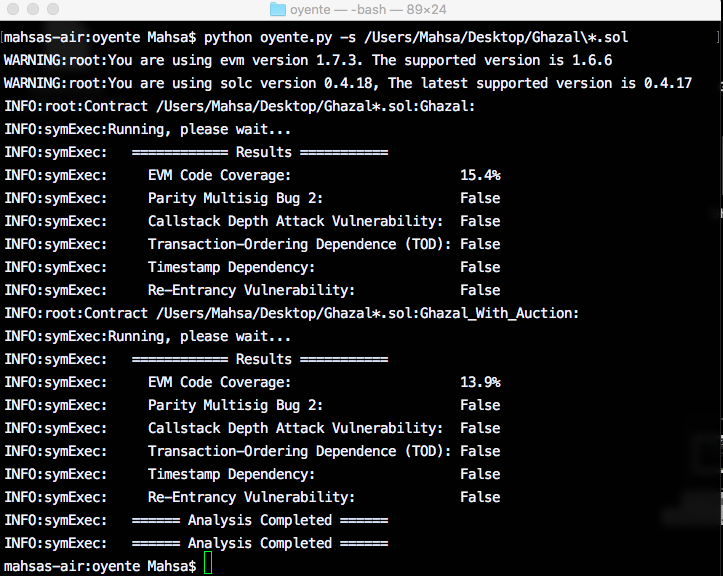
\includegraphics[width=0.8\textwidth]{fig/GhazalstarOyenteResult.png}
\caption{\footnotesize{Results of \Ghazalstar security analysis using Oyente~\cite{luu2016making}.}\label{fig:oyente}}
\end{figure}

Ethereum smart contracts, in particular the ones implemented in Solidity, are notorious for programming pitfalls. As they generally transfer and handle assets of considerable value, bugs in Solidity code could result in serious vulnerabilities which can be exploited by adversaries. We use standard defensive programming approaches, in particular around functions that transfer money (such as the auction function that refunds the security deposits), by using explicitly coded state machines and locks, and by not making state-changes after transfers. We also analyze \Ghazal and \Ghazalstar against Oyente, a symbolic execution tool proposed by Luu~\etal\cite{luu2016making} which looks for potential security bugs like the re-entry attack (infamously). The results of the security analysis represent that both of the smart contracts are not vulnerable to any known critical security issue (see Figure~\ref{fig:oyente}).

% = = = = = = = = = = = = = = = = = = = = = = = = = = = = = = = = = = = = = = = = = =

\section{Concluding Remarks}

We hope that \UA systems with programmability continue to be explored in the literature. There are many open problems to work on. First and foremost is understanding the scalability issues and how to minimize the amount of data a client browser needs to fetch for each domain lookup. Blockstack has done an excellent job on this issue for non-programmable contracts. Future work could also look at the layer above the smart contract: building web tools with user interfaces to enable interaction with the underlying functions. Finally, while auctions are one illustrative example of why programmability might be added to a PKI, we are sure there are many others. The modular design of \Ghazal using object-oriented programming should allow easy additions to our base contract, which we will provide as open source. Indeed, the auction itself in \Ghazalstar was added via inheritance and one function override (to enforce that ownership transfers, part of the parent class, could not be called during a live auction).  
 
\subsubsection*{Acknowledgements.} J. Clark thanks NSERC, FRQNT, and the Office of the Privacy Commissioner of Canada for funding that supported this research. 

































